% Options for packages loaded elsewhere
% Options for packages loaded elsewhere
\PassOptionsToPackage{unicode}{hyperref}
\PassOptionsToPackage{hyphens}{url}
\PassOptionsToPackage{dvipsnames,svgnames,x11names}{xcolor}
%
\documentclass[
  10pt,
]{report}
\usepackage{xcolor}
\usepackage[margin=0.7in]{geometry}
\usepackage{amsmath,amssymb}
\setcounter{secnumdepth}{5}
\usepackage{iftex}
\ifPDFTeX
  \usepackage[T1]{fontenc}
  \usepackage[utf8]{inputenc}
  \usepackage{textcomp} % provide euro and other symbols
\else % if luatex or xetex
  \usepackage{unicode-math} % this also loads fontspec
  \defaultfontfeatures{Scale=MatchLowercase}
  \defaultfontfeatures[\rmfamily]{Ligatures=TeX,Scale=1}
\fi
\usepackage{lmodern}
\ifPDFTeX\else
  % xetex/luatex font selection
  \setmainfont[]{Source Sans 3}
\fi
% Use upquote if available, for straight quotes in verbatim environments
\IfFileExists{upquote.sty}{\usepackage{upquote}}{}
\IfFileExists{microtype.sty}{% use microtype if available
  \usepackage[]{microtype}
  \UseMicrotypeSet[protrusion]{basicmath} % disable protrusion for tt fonts
}{}
\makeatletter
\@ifundefined{KOMAClassName}{% if non-KOMA class
  \IfFileExists{parskip.sty}{%
    \usepackage{parskip}
  }{% else
    \setlength{\parindent}{0pt}
    \setlength{\parskip}{6pt plus 2pt minus 1pt}}
}{% if KOMA class
  \KOMAoptions{parskip=half}}
\makeatother
% Make \paragraph and \subparagraph free-standing
\makeatletter
\ifx\paragraph\undefined\else
  \let\oldparagraph\paragraph
  \renewcommand{\paragraph}{
    \@ifstar
      \xxxParagraphStar
      \xxxParagraphNoStar
  }
  \newcommand{\xxxParagraphStar}[1]{\oldparagraph*{#1}\mbox{}}
  \newcommand{\xxxParagraphNoStar}[1]{\oldparagraph{#1}\mbox{}}
\fi
\ifx\subparagraph\undefined\else
  \let\oldsubparagraph\subparagraph
  \renewcommand{\subparagraph}{
    \@ifstar
      \xxxSubParagraphStar
      \xxxSubParagraphNoStar
  }
  \newcommand{\xxxSubParagraphStar}[1]{\oldsubparagraph*{#1}\mbox{}}
  \newcommand{\xxxSubParagraphNoStar}[1]{\oldsubparagraph{#1}\mbox{}}
\fi
\makeatother


\usepackage{longtable,booktabs,array}
\usepackage{calc} % for calculating minipage widths
% Correct order of tables after \paragraph or \subparagraph
\usepackage{etoolbox}
\makeatletter
\patchcmd\longtable{\par}{\if@noskipsec\mbox{}\fi\par}{}{}
\makeatother
% Allow footnotes in longtable head/foot
\IfFileExists{footnotehyper.sty}{\usepackage{footnotehyper}}{\usepackage{footnote}}
\makesavenoteenv{longtable}
\usepackage{graphicx}
\makeatletter
\newsavebox\pandoc@box
\newcommand*\pandocbounded[1]{% scales image to fit in text height/width
  \sbox\pandoc@box{#1}%
  \Gscale@div\@tempa{\textheight}{\dimexpr\ht\pandoc@box+\dp\pandoc@box\relax}%
  \Gscale@div\@tempb{\linewidth}{\wd\pandoc@box}%
  \ifdim\@tempb\p@<\@tempa\p@\let\@tempa\@tempb\fi% select the smaller of both
  \ifdim\@tempa\p@<\p@\scalebox{\@tempa}{\usebox\pandoc@box}%
  \else\usebox{\pandoc@box}%
  \fi%
}
% Set default figure placement to htbp
\def\fps@figure{htbp}
\makeatother





\setlength{\emergencystretch}{3em} % prevent overfull lines

\providecommand{\tightlist}{%
  \setlength{\itemsep}{0pt}\setlength{\parskip}{0pt}}



 


\usepackage{booktabs}
\usepackage{longtable}
\usepackage{array}
\usepackage{multirow}
\usepackage{wrapfig}
\usepackage{float}
\usepackage{colortbl}
\usepackage{pdflscape}
\usepackage{tabu}
\usepackage{threeparttable}
\usepackage{threeparttablex}
\usepackage[normalem]{ulem}
\usepackage{makecell}
\usepackage{xcolor}
\usepackage{geometry}
\usepackage{titlesec}
\usepackage{parskip}
\usepackage{setspace}
\onehalfspacing
\usepackage{fontspec}
\usepackage{booktabs}
\usepackage{longtable}
\usepackage{array}
\usepackage{multirow}
\usepackage{wrapfig}
\usepackage{float}
\usepackage{hyperref}
\hypersetup{colorlinks=true, linkcolor=blue, urlcolor=blue}
\usepackage{graphicx}
\usepackage{xcolor}
\definecolor{mygray}{HTML}{303538}
\makeatletter
\def\@titlepage{%
  \newpage
  \thispagestyle{empty}%
  \null
  \vfil
  \begin{center}%
    \let \footnote \thanks
    {\LARGE \textbf{\@title} \par\vskip 10\p@ }
    {\large \textit{\@subtitle} \par\vskip 10\p@ }
    \vskip 1em
    {\large \@author \par\vskip 1em}
    \vskip 1em
    {\large \@date \par}
    \vfil
  \end{center}
  \null
}
\makeatother
\AtBeginDocument{\color{mygray}}
\makeatletter
\@ifpackageloaded{caption}{}{\usepackage{caption}}
\AtBeginDocument{%
\ifdefined\contentsname
  \renewcommand*\contentsname{Table of contents}
\else
  \newcommand\contentsname{Table of contents}
\fi
\ifdefined\listfigurename
  \renewcommand*\listfigurename{List of Figures}
\else
  \newcommand\listfigurename{List of Figures}
\fi
\ifdefined\listtablename
  \renewcommand*\listtablename{List of Tables}
\else
  \newcommand\listtablename{List of Tables}
\fi
\ifdefined\figurename
  \renewcommand*\figurename{Figure}
\else
  \newcommand\figurename{Figure}
\fi
\ifdefined\tablename
  \renewcommand*\tablename{Table}
\else
  \newcommand\tablename{Table}
\fi
}
\@ifpackageloaded{float}{}{\usepackage{float}}
\floatstyle{ruled}
\@ifundefined{c@chapter}{\newfloat{codelisting}{h}{lop}}{\newfloat{codelisting}{h}{lop}[chapter]}
\floatname{codelisting}{Listing}
\newcommand*\listoflistings{\listof{codelisting}{List of Listings}}
\makeatother
\makeatletter
\makeatother
\makeatletter
\@ifpackageloaded{caption}{}{\usepackage{caption}}
\@ifpackageloaded{subcaption}{}{\usepackage{subcaption}}
\makeatother
\usepackage{bookmark}
\IfFileExists{xurl.sty}{\usepackage{xurl}}{} % add URL line breaks if available
\urlstyle{same}
\hypersetup{
  pdftitle={Institutional Capacity Assessment Report - Department of Agriculture and Rural Development},
  pdfauthor={Vanuatu Public Service Commission},
  colorlinks=true,
  linkcolor={blue},
  filecolor={Maroon},
  citecolor={Blue},
  urlcolor={Blue},
  pdfcreator={LaTeX via pandoc}}


\title{Institutional Capacity Assessment Report - Department of
Agriculture and Rural Development}
\usepackage{etoolbox}
\makeatletter
\providecommand{\subtitle}[1]{% add subtitle to \maketitle
  \apptocmd{\@title}{\par {\large #1 \par}}{}{}
}
\makeatother
\subtitle{Under the Ministry of Agriculture, Livestock, Forestry,
Fisheries and Biosecurity}
\author{Vanuatu Public Service Commission}
\date{2025-09-01}
\begin{document}
\maketitle

\renewcommand*\contentsname{Table of contents}
{
\hypersetup{linkcolor=}
\setcounter{tocdepth}{2}
\tableofcontents
}
\listoffigures
\listoftables


\maketitle

\chapter{Introduction}\label{introduction}

The National Sustainability Development Plan's (NSDP) society pillar
goal 6 provides for ``strong and effective institutions for ensuring a
dynamic public sector with good governance principles and strong
institutions delivering the support and services expected by all
citizens of Vanuatu''. OPSC's overall development program and policy
objectives for the work of individual or institutional capacity
assessment and development is also guided by this goal.

This report provides some background to the Institutional Capacity
Assessment process undertaken in August 2025 with the Department of
Agriculture and Rural Development staff and provides the results or
outcome of the assessment. The Department of Agriculture and Rural
Development is encouraged to review and verify the report, and make
appropriate plans to address any shortfall or improvements in
institutional capacity areas or elements identified through the
assessment.

\chapter{Background}\label{background}

\section{What is meant by ``capacity'' and ``capacity
development''?}\label{what-is-meant-by-capacity-and-capacity-development}

The phrase ``we need more capacity'' is often used to refer to: we don't
have enough staff; we need more training; our office space is too small;
our strategy is demanding more of us than what we can realistically
deliver; we need better systems of work; we need more efficient
processes; our infrastructure is outdated and needs replacement; we need
bigger budgets. Any of these statements are a reflection of capacity,
but none of them alone suffices a thorough definition of capacity.

`Capacity' is a commonly used term in the context of international,
organisational, and community development. However, when confronted with
institutional capacity development assessment and planning requirements,
it is important to have a shared understanding of what `capacity' means
to ensure effective development approaches. Key understanding can be
drawn from the following perspectives on the nature of capacity and
capacity development.

\textbf{On the nature of capacity\ldots{}}

\begin{quote}
``\ldots the ability of individuals, institutions, and societies to
perform functions, solve problems, and set and achieve objectives in a
sustainable manner.'' (United Nations Development Programme, 2010, p.~2)
\end{quote}

\textbf{On the development of capacity\ldots{}}

\begin{quote}
Capacity development involves much more than enhancing the knowledge and
skills of individuals. It depends crucially on the quality of the
organisations in which they work. In turn, the operations of particular
organisations are influenced by the enabling environment -- the
structures of power and influence and the institutions -- in which they
are embedded. Capacity is not only about skills and procedures; it is
also about incentives and governance. (OECD, 2008, p.~239)
\end{quote}

\begin{quote}
Capacity development is a locally driven process of learning by leaders,
coalitions and other agents of change that bring about changes in
socio-political, policy-related, and organizational factors to enhance
local ownership for and the effectiveness and efficiency of efforts to
achieve a development goal. (Otoo, Agapitova, \& Behrens, 2009, p.~3)
\end{quote}

So, capacity is about people, action, and results, all influenced by the
contexts and environments in which they operate. Capacity development is
therefore about learning and change that supports the achievement of
desired development results within that context and environment.
Institutional capacity development ultimately aims to increase the
ability of institutions to achieve the results for which they are
responsible.

\begin{figure}[H]

\caption{\label{fig-Capacity-people-context-environment}Capacity --
people, context \& environment}

\centering{

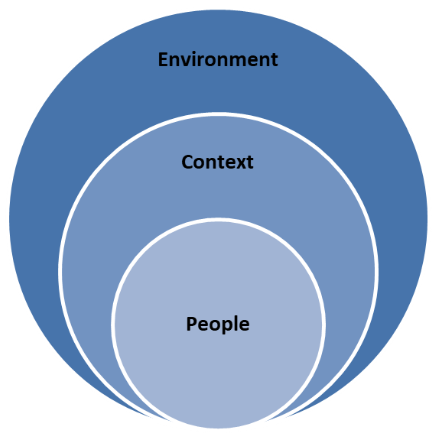
\includegraphics[width=3.125in,height=\textheight,keepaspectratio]{img/Capacity-people-context-environment.png}

}

\end{figure}%

It is important to understand the idea of ``capacity'' as an emergent
property and is ``living and dynamic'' (Fowler \& Ubels, 2010) rather
than as a fixed and easily measurable ``thing''. Capacity can manifest
in many ways: from an individual's choice to exercise a key skill to
achieve a task result, to a workgroup's ability to coordinate actions to
process a complex request, through to the coordinated delivery of public
services to the community.

\begin{figure}[H]

\caption{\label{fig-factors-influencing-capacity}Key factors influencing
`capacity'}

\centering{

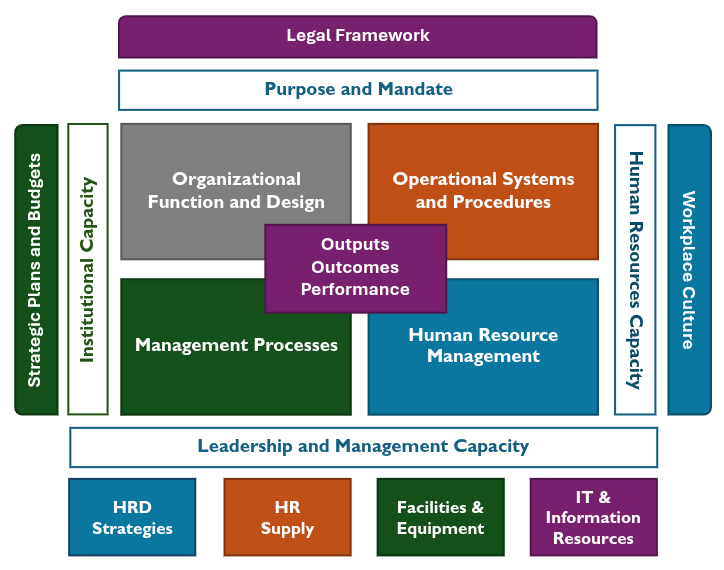
\includegraphics[width=4.16667in,height=\textheight,keepaspectratio]{img/factors-influencing-capacity.png}

}

\end{figure}%

Figure~\ref{fig-factors-influencing-capacity} provides important ideas
to guide the way we can examine and understand capacity and how capacity
might be developed in the line agencies of the public service. It seeks
to bring these ideas together, by identifying the key factors that are
likely to influence capacity and the development of capacity in this
context and environment:

At the highest strategic level, line agencies operate under particular
legal frameworks and national policies such as the NSDP that define
their powers and responsibilities that parts of their overall work
system hold, which is then reflected in the mandate and purpose of each
part. These in effect, define and bind what capacity is required of the
line agencies as a whole, and of each part.

Two key broad categories bound the capacity elements at the core:
institutional capacity, which is influenced by strategic plans and
budgets, and human resource capacity, which is influenced by the culture
and environment of the workplace. At the core are the institutional
elements of organisational design, operational systems, HRM, and
management processes, all of which influence the performance and
outcomes of the agency.

Underpinning all this is the capacity of institutions to demonstrate
effective leadership and management, together with key enabling elements
such as access to IT and information, facilities and equipment,
availability of human resources with required capabilities, and the
available options for targeted and specific human resource development.

In summary, the following key points are essential to consider when
planning for capacity development:

\begin{itemize}
\tightlist
\item
  Capacity is about the knowledge, skills, and abilities of people, and
  about what people can and will do together;
\item
  The primary driver for capacity concerns the strategic goals and
  purpose of the organisation, so all development planning must consider
  how well existing capacity serves these needs, which is what drives
  the need for assessment;
\item
  Changes in capacity should be measurable through achievement of
  planned activities, outputs, and outcomes, and ultimately impacts in
  the community through the line agencies' service delivery;
\item
  Capacity development is a long-term process -- it takes time,
  resources, and perseverance;
\item
  Capacity is an emergent property of an overall work system, and many
  factors contribute to capacity, how capacity emerges, and what can be
  achieved, so sensitivity and acute observation are needed to ensure
  that development is timely and appropriate.
\end{itemize}

\chapter{Institutional Capacity Assessment
Grid}\label{institutional-capacity-assessment-grid}

\section{How Department of Agriculture and Rural Development's
institutional capacity was
assessed}\label{how-department-of-agriculture-and-rural-developments-institutional-capacity-was-assessed}

OPSC's Framework for Institutional Capacity Assessment and Development
(see Appendix A) is designed to clarify the capacity needs, and
assessment and development approach that is relevant at the level of the
Institution or Agency. The focus is on institutional capacity targeting
organisational design, HRM, operational systems, leadership and
management practice, facilities and equipment, and the effectiveness of
the organisation in coordinating action to achieve operational and
development objectives.

The assessment framework and descriptions are based on a range of
sources that describe aspects of effective organisational functioning
that have been adapted to the unique Vanuatu Public Sector context.

The objectives of the ICAG, which can be used by staff and stakeholders
alike, include:

\begin{itemize}
\tightlist
\item
  To identify those particular areas of capacity that are strongest and
  those that need improvement;
\item
  To assess changes in an institution's capacity over time by
  readministering the ICAG;
\item
  To draw out different views within an organisation regarding capacity.
  Different responses to the ICAG amongst staff, stakeholders, and
  donors, for example, can be a valuable discussion starter within an
  organisation.
\end{itemize}

This assessment examined a range of institutional capacity elements
within the Department of Agriculture and Rural Development. A total of
eleven (11) Department of Agriculture and Rural Development staff
completed the institutional capacity assessment in August 2025.

The primary tool used to undertake the assessment is the Institutional
Capacity Assessment Grid (ICAG), a diagnostic tool that has been
developed and tailored to capture key data about capacity that is
relevant to line agencies or institutions. The ICAG asks the reader to
score the organisation on each element of organisational capacity
provided, by selecting the text that best describes the organisation's
current status or performance.

The ICAG itself is not a scientific tool, and should not be used as one.
It is difficult to quantify the different dimensions of capacity, and
therefore the different descriptive text is intended to be indicative
rather than exact. In this way, the scores are meant to provide an
indication of the ``temperature'' of the organisation's capacity in
order to identify areas of improvement.

The tool is meant to be a starting point for conversation leading to
capacity development planning. The 5 steps in the process are described
in the following diagram.

\begin{figure}[H]

\caption{\label{fig-five-steps-assessing-planning-capacity-development}Five-Step
Process for Assessing and Planning Capacity Development Using the ICAG}

\centering{

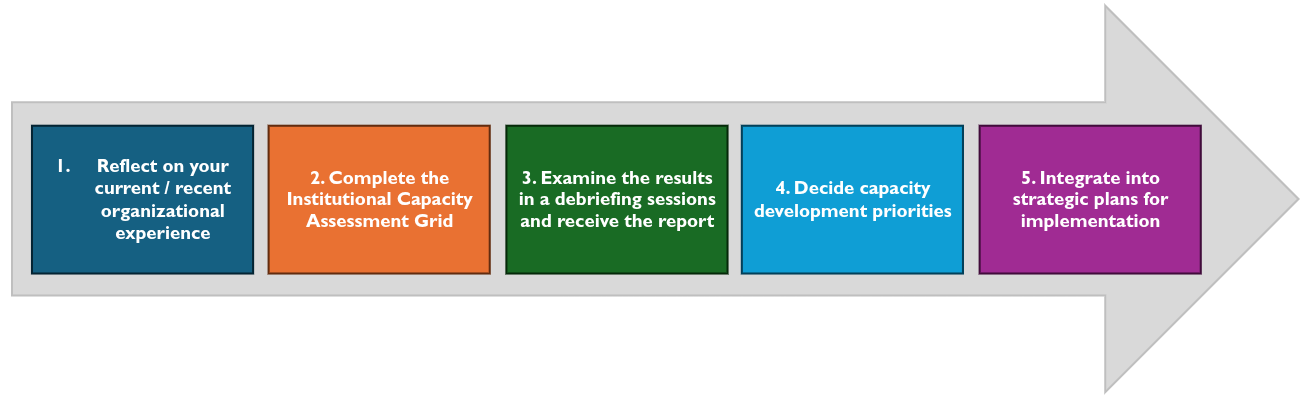
\includegraphics[width=5.20833in,height=\textheight,keepaspectratio]{img/five-steps-assessing-planning-capacity-development.png}

}

\end{figure}%

This report supports Step 3, and is intended to encourage closer
examination of key capacity areas that can then become the focus of
capacity development. The ICAG is also designed to help the members of
individual agencies reflect on and assess their own organisational
capacity.

The results of the ICAG can be used in many ways:

\begin{itemize}
\tightlist
\item
  To define key development priorities for line agencies;
\item
  To establish a ``baseline'' for organisational capacity and identify
  common development issues across line agencies and sectors;
\item
  Lastly, to identify where additional program supports from the OPSC or
  from development or donor partners could be offered to best effect.
\end{itemize}

\section{Methodology}\label{methodology}

\subsection{Data Collection}\label{data-collection}

The Institutional Capacity Assessment Grid (ICAG) was used to gather
information about the organizational capacity of different departments
within the Vanuatu Public Sector, including the Department of
Agriculture and Rural Development. This tool helps evaluate key areas
like organizational design, human resource management, operational
systems, leadership practices, and infrastructure. The survey was
conducted using Microsoft Office 365 Forms. They rated 31 capacity
categories on a scale from 1 (Clear Need) to 4 (High) based on
statements that described how well the department was performing (e.g.,
from ``little shared understanding'' to ``clear and compelling
vision'').

The survey responses were collected through Microsoft Office 365 Forms
and saved into a spreadsheet. This file included answers from various
departments, such as the Department of Agriculture and Rural Development
and the Department of Water Resources. Each row in the spreadsheet
represents one respondent, with details like their ID, email, name,
province, ministry, department, and their ratings for the 31 capacity
categories, written as descriptive text based on their chosen score.

\subsection{Data Processing}\label{data-processing}

The following steps were undertaken:

The information from the survey was prepared for analysis. Here's what
was done:

\begin{enumerate}
\def\labelenumi{\arabic{enumi}.}
\tightlist
\item
  \textbf{Data Extraction}: The survey responses were changed into a
  format that could be easily analyzed.
\item
  \textbf{Data Cleaning}: The text answers (e.g., ``little shared
  understanding'') were turned into numbers based on the ICAG scale:

  \begin{itemize}
  \tightlist
  \item
    A = 1 (Clear Need)
  \item
    B = 2 (Basic)
  \item
    C = 3 (Moderate)
  \item
    D = 4 (High) The first letter of each response was used to assign
    the correct number. If a response was missing or unclear, it was
    marked as missing and handled later.
  \end{itemize}
\end{enumerate}

\subsection{Data Analysis}\label{data-analysis}

The prepared data was analyzed using R to understand the Department of
Agriculture and Rural Development's institutional capacity. The process
included the following steps:

\begin{enumerate}
\def\labelenumi{\arabic{enumi}.}
\tightlist
\item
  \textbf{Loading the Dataset}: The survey data was brought into
  R\footnote{See Appendix A for detailed steps and the R code used in
    the analysis.}, and only the responses from the Department of
  Agriculture and Rural Development were selected.
\item
  \textbf{Calculating Mean Scores}: We figured out the average scores
  for each of the 31 capacity categories based on the Department of
  Agriculture and Rural Development's responses.
\item
  \textbf{Identifying Strongest and Weakest Capacities}: The top two
  categories with the highest average scores were noted as the
  strongest, and categories with averages of 2 or lower were marked as
  the weakest.
\item
  \textbf{Rating Distribution}: We counted how many times each score (1
  to 4) appeared for each capacity category.
\item
  \textbf{Visualization Data}: The average scores were prepared for
  charts, with one chart showing categories from most to least developed
  and another from least to most developed.
\item
  \textbf{Visualization}: charts were created using R. The first shows
  average scores ordered from most to least developed, and the second
  ranks them from least to most developed, using colors to highlight the
  scores and lines to show different levels of need.
\end{enumerate}

\subsection{How the ICAG Scale and Analysis Methods Were
Chosen}\label{how-the-icag-scale-and-analysis-methods-were-chosen}

The Institutional Capacity Assessment Grid (ICAG) scale, ranging from 1
to 4, was carefully designed to reflect the varying levels of
organizational capacity within the Vanuatu Public Sector, including the
Department of Agriculture and Rural Development. This scale---where 1
represents ``Clear Need,'' 2 indicates ``Basic,'' 3 denotes
``Moderate,'' and 4 signifies ``High''---was developed based on
qualitative descriptors tailored to the local context, drawing from
established organizational development frameworks. The descriptors for
each level (e.g., ``little shared understanding'' for 1, ``clear and
compelling vision'' for 4) were crafted to capture the spectrum of
performance across 31 capacity categories, ensuring relevance to the
department's operational and strategic challenges.

The analysis methods, including the calculation of mean scores and the
establishment of thresholds for identifying weakest capacities, were
selected to provide a robust, evidence-based foundation for actionable
priorities. Mean scores were computed by averaging the ratings provided
by the 11 Department of Agriculture and Rural Development staff who
participated in the August 2025 assessment, offering a reliable
aggregate measure of capacity across each category. The threshold of ≤ 2
was chosen to flag capacities requiring urgent attention, as scores at
or below this level indicate performance that is either at ``Clear
Need'' or just reaching ``Basic,'' signaling significant gaps that
hinder effective service delivery and strategic goal attainment. This
cutoff was determined to align with the National Sustainability
Development Plan's (NSDP) goal of strengthening public institutions,
ensuring that the Department of Agriculture and Rural Development can
prioritize resource allocation and capacity-building efforts where they
are most needed. This approach enables the department to focus on
critical areas, such as infrastructure or responsiveness, while
supporting long-term planning and improvement.

\section{Overview of results}\label{overview-of-results}

As a public institution with a broad scope and mandate for implementing
the national government's priorities, the MALFFB Corporate Plan, the
Department Business Plan, and other priorities of the National
Sustainability Development Plan (NSDP), the Department of Agriculture
and Rural Development acknowledges its challenges, including limited
financial and human resources. The Department has undertaken to shift
its approach toward working closely with, and harnessing the available
resources offered through other government line agencies, as well as
credible non-government, civil, and faith-based organizations. This
shift necessitates the development and consolidation of specific skills
and capacities.

To build an evidence base for capacity development to support this
transition, staff from the Department of Agriculture and Rural
Development participated in an institutional capacity assessment
activity conducted by the Office of the Public Service Commission (OPSC)
in August 2025. The assessment, based on the Institutional Capacity
Assessment Grid (ICAG), involved 11 staff members and evaluated 31
capacity categories to identify strengths and areas for improvement.

The analysis reveals that the Department of Agriculture and Rural
Development excels in strategic planning and mission clarity, with mean
scores reflecting a moderate to high capacity in these areas. However,
critical gaps persist in infrastructure, responsiveness to environmental
changes, and financial management, necessitating targeted interventions
to enhance overall performance. These findings provide a foundation for
the Department to prioritize resource allocation and capacity-building
efforts, aligning with the NSDP's goal of strengthening public
institutions.

\begin{figure}[H]

\caption{\label{fig-summary-bar}Summary of results by category
(institutional average)}

\centering{

\pandocbounded{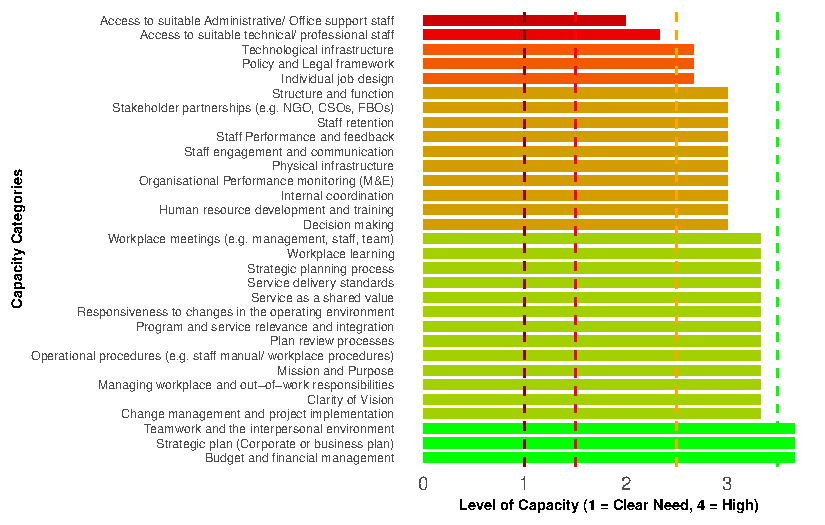
\includegraphics[keepaspectratio]{ICA_Report_Template_files/figure-pdf/fig-summary-bar-1.pdf}}

}

\end{figure}%

\subsection{Strongest Capacities}\label{strongest-capacities}

Based on Figure 3, capacities that indicate a moderate to high level
include:

\begin{itemize}
\tightlist
\item
  \textbf{Mission and Purpose}, described as, ``Clear expression of
  organisation's reason for existence which reflects its purpose and
  values; held by many within the organisation and referred to often''.
\item
  \textbf{Strategic plan (Corporate or business plan)}, described as,
  ``The plan is in place, is up to date and links well to the mission;
  Most strategies in the plan have been developed into clear projects
  with budgets and activities well defined to guide work and program
  planning; Most staff are aware of the plan, use it and were consulted
  when it was developed; Plans are used to guide management decisions''.
\end{itemize}

\begingroup\fontsize{8}{10}\selectfont

\begin{longtable}[t]{>{\raggedright\arraybackslash}p{7cm}rl}
\caption{\label{tab:unnamed-chunk-6}Summary of Strongest and Weakest Capacities}\\
\toprule
\textbf{Capacity Category} & \textbf{Mean Score} & \textbf{Type}\\
\midrule
Decision making & 3.6 & Strongest\\
Teamwork and the interpersonal environment & 3.6 & Strongest\\
\bottomrule
\end{longtable}
\endgroup{}

\subsection{Top 10 Development Priorities and
Recommendations}\label{top-10-development-priorities-and-recommendations}

The OPSC analysis identifies the following 10 capacity areas as
priorities for development, based on mean scores ≤ 2.5, indicating
performance at or below the ``Basic'' level. These priorities are
critical for the Department of Agriculture and Rural Development to
address to enhance institutional effectiveness and align with NSDP
goals. Recommended actions are provided to guide decision-making and
resource allocation.

\begingroup\fontsize{8}{10}\selectfont

\begin{longtable}[t]{lr>{\raggedright\arraybackslash}p{7cm}}
\caption{\label{tab:unnamed-chunk-7}Development Priorities and Recommendations}\\
\toprule
\textbf{Capacity Category} & \textbf{Mean Score} & \textbf{Recommended Action}\\
\midrule
Human resource development and training & 2.2 & Develop a clear vision statement through staff workshops\\
Clarity of Vision & 2.4 & Review and update policy/legal framework with legal experts\\
Responsiveness to changes in the operating environment & 2.4 & Implement training on environmental responsiveness\\
Operational procedures (e.g. staff manual/ workplace procedures) & 2.4 & Establish an inclusive strategic planning committee\\
Organisational Performance monitoring (M\&E) & 2.4 & Introduce regular plan review schedules\\
\bottomrule
\end{longtable}
\endgroup{}

\subsection{Capacities Requiring Urgent
Development}\label{capacities-requiring-urgent-development}

Among the top 10 priorities, Managing workplace and out-of-work
responsibilities stands out as a capacity with a mean score indicating
``Clear Need,'' characterized by, ``Staff find it difficult to attend
work and to achieve the required work hours; They feel very pulled in
the direction of their out-of-work responsibilities. Characterised by
high levels of unauthorised absence, usually unexplained; Management
recognise the problems but fail to take action and don't hold staff
accountable for absences.'' This area requires immediate action,
alongside the other nine priorities listed in the table, to raise
performance to at least a ``Moderate'' level and support the
Department's strategic objectives.

\chapter{Appendix A: OPSC's Framework for Institutional Capacity
Assessment and
Development}\label{appendix-a-opscs-framework-for-institutional-capacity-assessment-and-development}

(Placeholder for Appendix A content)

\chapter{Appendix B: Planning for Institutional Capacity
Development}\label{appendix-b-planning-for-institutional-capacity-development}

The following process is offered as a means by which Department of
Agriculture and Rural Development can:

\begin{itemize}
\tightlist
\item
  Make sense of the results of the ICAG
\item
  Identify key priorities and strategies to address capacity needs, and
\item
  Ensure where necessary that the strategies are captured in 2020 and
  onwards business plans.
\end{itemize}

\textbf{Step 1: Gather a group of senior staff to examine the results}

Move gradually through the report, step by step, taking time to explore
any anomalies or results that are surprising or unexpected.

\textbf{Step 2: Identify the key ideas for capacity development}

Section 3.3 of the report lays out the priorities based on the analysis
of the data from the assessment process. The ``thermometer'' indicates
the current level of capacity according to the results, and the
accompanying text provides the descriptors from the ICAG questionnaire
to help identify possible development directions. Taking into
consideration the recommendations made, work through each one in turn
and ask:

\begin{itemize}
\tightlist
\item
  What can we realistically do in the next 12 months and onwards to
  develop capacity in this area?
\item
  Will we need additional resources to do this? If so, where will the
  resources be sourced from?
\item
  What kind of changes will this require of us? What will we need to
  keep doing? Stop doing? Start doing?
\item
  How will the changes be embedded institutionally, into policies,
  procedures, or systems of work?
\item
  How will we know if our efforts have been successful in developing
  greater capacity? (M\&E)
\end{itemize}

\textbf{Step 3: Decide the preferred strategies and integrate into the
2020 Business Plan and subsequent plans.}

This step is an important part of recognising the importance of the
change that is needed by embedding it into the priorities for 2020 and
subsequent years. Inclusion in annual business plans will also ensure
that the work is budgeted for and that progress is monitored as part of
the plan review.

\chapter{Appendix C: List of
References}\label{appendix-c-list-of-references}

(Placeholder for Appendix C content)




\end{document}
